% Options for packages loaded elsewhere
\PassOptionsToPackage{unicode}{hyperref}
\PassOptionsToPackage{hyphens}{url}
\PassOptionsToPackage{dvipsnames,svgnames,x11names}{xcolor}
%
\documentclass[
  letterpaper,
  DIV=11]{scrartcl}

\usepackage{amsmath,amssymb}
\usepackage{iftex}
\ifPDFTeX
  \usepackage[T1]{fontenc}
  \usepackage[utf8]{inputenc}
  \usepackage{textcomp} % provide euro and other symbols
\else % if luatex or xetex
  \usepackage{unicode-math}
  \defaultfontfeatures{Scale=MatchLowercase}
  \defaultfontfeatures[\rmfamily]{Ligatures=TeX,Scale=1}
\fi
\usepackage{lmodern}
\ifPDFTeX\else  
    % xetex/luatex font selection
\fi
% Use upquote if available, for straight quotes in verbatim environments
\IfFileExists{upquote.sty}{\usepackage{upquote}}{}
\IfFileExists{microtype.sty}{% use microtype if available
  \usepackage[]{microtype}
  \UseMicrotypeSet[protrusion]{basicmath} % disable protrusion for tt fonts
}{}
\makeatletter
\@ifundefined{KOMAClassName}{% if non-KOMA class
  \IfFileExists{parskip.sty}{%
    \usepackage{parskip}
  }{% else
    \setlength{\parindent}{0pt}
    \setlength{\parskip}{6pt plus 2pt minus 1pt}}
}{% if KOMA class
  \KOMAoptions{parskip=half}}
\makeatother
\usepackage{xcolor}
\setlength{\emergencystretch}{3em} % prevent overfull lines
\setcounter{secnumdepth}{5}
% Make \paragraph and \subparagraph free-standing
\ifx\paragraph\undefined\else
  \let\oldparagraph\paragraph
  \renewcommand{\paragraph}[1]{\oldparagraph{#1}\mbox{}}
\fi
\ifx\subparagraph\undefined\else
  \let\oldsubparagraph\subparagraph
  \renewcommand{\subparagraph}[1]{\oldsubparagraph{#1}\mbox{}}
\fi

\usepackage{color}
\usepackage{fancyvrb}
\newcommand{\VerbBar}{|}
\newcommand{\VERB}{\Verb[commandchars=\\\{\}]}
\DefineVerbatimEnvironment{Highlighting}{Verbatim}{commandchars=\\\{\}}
% Add ',fontsize=\small' for more characters per line
\usepackage{framed}
\definecolor{shadecolor}{RGB}{241,243,245}
\newenvironment{Shaded}{\begin{snugshade}}{\end{snugshade}}
\newcommand{\AlertTok}[1]{\textcolor[rgb]{0.68,0.00,0.00}{#1}}
\newcommand{\AnnotationTok}[1]{\textcolor[rgb]{0.37,0.37,0.37}{#1}}
\newcommand{\AttributeTok}[1]{\textcolor[rgb]{0.40,0.45,0.13}{#1}}
\newcommand{\BaseNTok}[1]{\textcolor[rgb]{0.68,0.00,0.00}{#1}}
\newcommand{\BuiltInTok}[1]{\textcolor[rgb]{0.00,0.23,0.31}{#1}}
\newcommand{\CharTok}[1]{\textcolor[rgb]{0.13,0.47,0.30}{#1}}
\newcommand{\CommentTok}[1]{\textcolor[rgb]{0.37,0.37,0.37}{#1}}
\newcommand{\CommentVarTok}[1]{\textcolor[rgb]{0.37,0.37,0.37}{\textit{#1}}}
\newcommand{\ConstantTok}[1]{\textcolor[rgb]{0.56,0.35,0.01}{#1}}
\newcommand{\ControlFlowTok}[1]{\textcolor[rgb]{0.00,0.23,0.31}{#1}}
\newcommand{\DataTypeTok}[1]{\textcolor[rgb]{0.68,0.00,0.00}{#1}}
\newcommand{\DecValTok}[1]{\textcolor[rgb]{0.68,0.00,0.00}{#1}}
\newcommand{\DocumentationTok}[1]{\textcolor[rgb]{0.37,0.37,0.37}{\textit{#1}}}
\newcommand{\ErrorTok}[1]{\textcolor[rgb]{0.68,0.00,0.00}{#1}}
\newcommand{\ExtensionTok}[1]{\textcolor[rgb]{0.00,0.23,0.31}{#1}}
\newcommand{\FloatTok}[1]{\textcolor[rgb]{0.68,0.00,0.00}{#1}}
\newcommand{\FunctionTok}[1]{\textcolor[rgb]{0.28,0.35,0.67}{#1}}
\newcommand{\ImportTok}[1]{\textcolor[rgb]{0.00,0.46,0.62}{#1}}
\newcommand{\InformationTok}[1]{\textcolor[rgb]{0.37,0.37,0.37}{#1}}
\newcommand{\KeywordTok}[1]{\textcolor[rgb]{0.00,0.23,0.31}{#1}}
\newcommand{\NormalTok}[1]{\textcolor[rgb]{0.00,0.23,0.31}{#1}}
\newcommand{\OperatorTok}[1]{\textcolor[rgb]{0.37,0.37,0.37}{#1}}
\newcommand{\OtherTok}[1]{\textcolor[rgb]{0.00,0.23,0.31}{#1}}
\newcommand{\PreprocessorTok}[1]{\textcolor[rgb]{0.68,0.00,0.00}{#1}}
\newcommand{\RegionMarkerTok}[1]{\textcolor[rgb]{0.00,0.23,0.31}{#1}}
\newcommand{\SpecialCharTok}[1]{\textcolor[rgb]{0.37,0.37,0.37}{#1}}
\newcommand{\SpecialStringTok}[1]{\textcolor[rgb]{0.13,0.47,0.30}{#1}}
\newcommand{\StringTok}[1]{\textcolor[rgb]{0.13,0.47,0.30}{#1}}
\newcommand{\VariableTok}[1]{\textcolor[rgb]{0.07,0.07,0.07}{#1}}
\newcommand{\VerbatimStringTok}[1]{\textcolor[rgb]{0.13,0.47,0.30}{#1}}
\newcommand{\WarningTok}[1]{\textcolor[rgb]{0.37,0.37,0.37}{\textit{#1}}}

\providecommand{\tightlist}{%
  \setlength{\itemsep}{0pt}\setlength{\parskip}{0pt}}\usepackage{longtable,booktabs,array}
\usepackage{calc} % for calculating minipage widths
% Correct order of tables after \paragraph or \subparagraph
\usepackage{etoolbox}
\makeatletter
\patchcmd\longtable{\par}{\if@noskipsec\mbox{}\fi\par}{}{}
\makeatother
% Allow footnotes in longtable head/foot
\IfFileExists{footnotehyper.sty}{\usepackage{footnotehyper}}{\usepackage{footnote}}
\makesavenoteenv{longtable}
\usepackage{graphicx}
\makeatletter
\def\maxwidth{\ifdim\Gin@nat@width>\linewidth\linewidth\else\Gin@nat@width\fi}
\def\maxheight{\ifdim\Gin@nat@height>\textheight\textheight\else\Gin@nat@height\fi}
\makeatother
% Scale images if necessary, so that they will not overflow the page
% margins by default, and it is still possible to overwrite the defaults
% using explicit options in \includegraphics[width, height, ...]{}
\setkeys{Gin}{width=\maxwidth,height=\maxheight,keepaspectratio}
% Set default figure placement to htbp
\makeatletter
\def\fps@figure{htbp}
\makeatother
\newlength{\cslhangindent}
\setlength{\cslhangindent}{1.5em}
\newlength{\csllabelwidth}
\setlength{\csllabelwidth}{3em}
\newlength{\cslentryspacingunit} % times entry-spacing
\setlength{\cslentryspacingunit}{\parskip}
\newenvironment{CSLReferences}[2] % #1 hanging-ident, #2 entry spacing
 {% don't indent paragraphs
  \setlength{\parindent}{0pt}
  % turn on hanging indent if param 1 is 1
  \ifodd #1
  \let\oldpar\par
  \def\par{\hangindent=\cslhangindent\oldpar}
  \fi
  % set entry spacing
  \setlength{\parskip}{#2\cslentryspacingunit}
 }%
 {}
\usepackage{calc}
\newcommand{\CSLBlock}[1]{#1\hfill\break}
\newcommand{\CSLLeftMargin}[1]{\parbox[t]{\csllabelwidth}{#1}}
\newcommand{\CSLRightInline}[1]{\parbox[t]{\linewidth - \csllabelwidth}{#1}\break}
\newcommand{\CSLIndent}[1]{\hspace{\cslhangindent}#1}

\usepackage{booktabs}
\usepackage{longtable}
\usepackage{array}
\usepackage{multirow}
\usepackage{wrapfig}
\usepackage{float}
\usepackage{colortbl}
\usepackage{pdflscape}
\usepackage{tabu}
\usepackage{threeparttable}
\usepackage{threeparttablex}
\usepackage[normalem]{ulem}
\usepackage{makecell}
\usepackage{xcolor}
\KOMAoption{captions}{tableheading}
\makeatletter
\@ifpackageloaded{tcolorbox}{}{\usepackage[skins,breakable]{tcolorbox}}
\@ifpackageloaded{fontawesome5}{}{\usepackage{fontawesome5}}
\definecolor{quarto-callout-color}{HTML}{909090}
\definecolor{quarto-callout-note-color}{HTML}{0758E5}
\definecolor{quarto-callout-important-color}{HTML}{CC1914}
\definecolor{quarto-callout-warning-color}{HTML}{EB9113}
\definecolor{quarto-callout-tip-color}{HTML}{00A047}
\definecolor{quarto-callout-caution-color}{HTML}{FC5300}
\definecolor{quarto-callout-color-frame}{HTML}{acacac}
\definecolor{quarto-callout-note-color-frame}{HTML}{4582ec}
\definecolor{quarto-callout-important-color-frame}{HTML}{d9534f}
\definecolor{quarto-callout-warning-color-frame}{HTML}{f0ad4e}
\definecolor{quarto-callout-tip-color-frame}{HTML}{02b875}
\definecolor{quarto-callout-caution-color-frame}{HTML}{fd7e14}
\makeatother
\makeatletter
\makeatother
\makeatletter
\makeatother
\makeatletter
\@ifpackageloaded{caption}{}{\usepackage{caption}}
\AtBeginDocument{%
\ifdefined\contentsname
  \renewcommand*\contentsname{Inhaltsverzeichnis}
\else
  \newcommand\contentsname{Inhaltsverzeichnis}
\fi
\ifdefined\listfigurename
  \renewcommand*\listfigurename{Abbildungsverzeichnis}
\else
  \newcommand\listfigurename{Abbildungsverzeichnis}
\fi
\ifdefined\listtablename
  \renewcommand*\listtablename{Tabellenverzeichnis}
\else
  \newcommand\listtablename{Tabellenverzeichnis}
\fi
\ifdefined\figurename
  \renewcommand*\figurename{Abbildung}
\else
  \newcommand\figurename{Abbildung}
\fi
\ifdefined\tablename
  \renewcommand*\tablename{Tabelle}
\else
  \newcommand\tablename{Tabelle}
\fi
}
\@ifpackageloaded{float}{}{\usepackage{float}}
\floatstyle{ruled}
\@ifundefined{c@chapter}{\newfloat{codelisting}{h}{lop}}{\newfloat{codelisting}{h}{lop}[chapter]}
\floatname{codelisting}{Listing}
\newcommand*\listoflistings{\listof{codelisting}{Listingverzeichnis}}
\makeatother
\makeatletter
\@ifpackageloaded{caption}{}{\usepackage{caption}}
\@ifpackageloaded{subcaption}{}{\usepackage{subcaption}}
\makeatother
\makeatletter
\@ifpackageloaded{tcolorbox}{}{\usepackage[skins,breakable]{tcolorbox}}
\makeatother
\makeatletter
\@ifundefined{shadecolor}{\definecolor{shadecolor}{rgb}{.97, .97, .97}}
\makeatother
\makeatletter
\makeatother
\makeatletter
\makeatother
\makeatletter
\@ifpackageloaded{tikz}{}{\usepackage{tikz}}
\makeatother
        \newcommand*\circled[1]{\tikz[baseline=(char.base)]{
          \node[shape=circle,draw,inner sep=1pt] (char) {{\scriptsize#1}};}}  
                  
\ifLuaTeX
\usepackage[bidi=basic]{babel}
\else
\usepackage[bidi=default]{babel}
\fi
\babelprovide[main,import]{ngerman}
% get rid of language-specific shorthands (see #6817):
\let\LanguageShortHands\languageshorthands
\def\languageshorthands#1{}
\ifLuaTeX
  \usepackage{selnolig}  % disable illegal ligatures
\fi
\IfFileExists{bookmark.sty}{\usepackage{bookmark}}{\usepackage{hyperref}}
\IfFileExists{xurl.sty}{\usepackage{xurl}}{} % add URL line breaks if available
\urlstyle{same} % disable monospaced font for URLs
\hypersetup{
  pdftitle={Deskriptive Statistik},
  pdfauthor={Daniela Palleschi},
  pdflang={de},
  colorlinks=true,
  linkcolor={blue},
  filecolor={Maroon},
  citecolor={Blue},
  urlcolor={Blue},
  pdfcreator={LaTeX via pandoc}}

\title{Deskriptive Statistik}
\usepackage{etoolbox}
\makeatletter
\providecommand{\subtitle}[1]{% add subtitle to \maketitle
  \apptocmd{\@title}{\par {\large #1 \par}}{}{}
}
\makeatother
\subtitle{Maße der zentralen Tendenz und Streuung}
\author{Daniela Palleschi}
\date{2023-06-13}

\begin{document}
\maketitle
\ifdefined\Shaded\renewenvironment{Shaded}{\begin{tcolorbox}[interior hidden, breakable, boxrule=0pt, sharp corners, enhanced, borderline west={3pt}{0pt}{shadecolor}, frame hidden]}{\end{tcolorbox}}\fi

\renewcommand*\contentsname{Inhaltsverzeichnis}
{
\hypersetup{linkcolor=}
\setcounter{tocdepth}{3}
\tableofcontents
}
\hypertarget{wiederholung}{%
\section*{Wiederholung}\label{wiederholung}}
\addcontentsline{toc}{section}{Wiederholung}

Letzte Woche haben wir\ldots{}

\begin{itemize}
\tightlist
\item
  etwas über breite und lange Daten gelernt ✅
\item
  breite Daten länger gemacht ✅
\item
  lange Daten breiter gemacht ✅
\end{itemize}

\hypertarget{uxfcberpruxfcfung}{%
\subsection{Überprüfung}\label{uxfcberpruxfcfung}}

\begin{Shaded}
\begin{Highlighting}[]
\NormalTok{pacman}\SpecialCharTok{::}\FunctionTok{p\_load}\NormalTok{(tidyverse,}
\NormalTok{               here)}
\end{Highlighting}
\end{Shaded}

\begin{Shaded}
\begin{Highlighting}[]
\NormalTok{df\_biondo }\OtherTok{\textless{}{-}} \FunctionTok{read\_csv}\NormalTok{(}\FunctionTok{here}\NormalTok{(}\StringTok{"daten"}\NormalTok{, }\StringTok{"biondo\_etal\_2021\_tidy.csv"}\NormalTok{))}
\NormalTok{df\_billboard }\OtherTok{\textless{}{-}} \FunctionTok{read\_csv}\NormalTok{(}\FunctionTok{here}\NormalTok{(}\StringTok{"daten"}\NormalTok{, }\StringTok{"billboard.csv"}\NormalTok{))}
\end{Highlighting}
\end{Shaded}

\hypertarget{annotated-cell-1}{%
\label{annotated-cell-1}}%
\begin{Shaded}
\begin{Highlighting}[]
\NormalTok{df\_biondo }\SpecialCharTok{\%\textgreater{}\%} \hspace*{\fill}\NormalTok{\circled{1}}
  \FunctionTok{head}\NormalTok{(}\AttributeTok{n =} \DecValTok{5}\NormalTok{) }\SpecialCharTok{\%\textgreater{}\%} \hspace*{\fill}\NormalTok{\circled{2}}
\NormalTok{  knitr}\SpecialCharTok{::}\FunctionTok{kable}\NormalTok{() }\SpecialCharTok{\%\textgreater{}\%} \hspace*{\fill}\NormalTok{\circled{3}}
\NormalTok{  kableExtra}\SpecialCharTok{::}\FunctionTok{kable\_styling}\NormalTok{(}\AttributeTok{font\_size =} \DecValTok{20}\NormalTok{) }\hspace*{\fill}\NormalTok{\circled{4}}
\end{Highlighting}
\end{Shaded}

\begin{description}
\tightlist
\item[\circled{1}]
Take the data frame \texttt{df\_biondo}, and then
\item[\circled{2}]
take just the first 5 rows, and then
\item[\circled{3}]
create a pretty \texttt{knitr} table, and then
\item[\circled{4}]
make the table even nicer using \texttt{kableExtra}, with font size 20
\end{description}

\begin{table}
\centering\begingroup\fontsize{20}{22}\selectfont

\begin{tabular}{r|r|l|l|r|r|r|r}
\hline
subj & item & tense & verb & gramm & acc & rt & tt\\
\hline
1 & 1 & future & representarán & 1 & 1 & 840.1917 & 1596\\
\hline
1 & 2 & future & alzarán & 1 & 1 & 1310.1809 & 648\\
\hline
1 & 3 & future & centrarán & 1 & 1 & 700.2674 & 841\\
\hline
1 & 4 & future & coleccionarán & 1 & 1 & 650.1856 & 1337\\
\hline
1 & 5 & future & complementarán & 1 & 1 & 580.2159 & 1400\\
\hline
\end{tabular}
\endgroup{}
\end{table}

\begin{itemize}
\tightlist
\item
  we usually don't want to save the output from \texttt{head()},
  \texttt{knitr::kable()} and \texttt{kableExtra::kable\_styling()} as
  an object

  \begin{itemize}
  \tightlist
  \item
    and certainly not as an object that begins with \texttt{df\_}, which
    stands for \texttt{dataframe}
  \end{itemize}
\end{itemize}

\begin{center}\rule{0.5\linewidth}{0.5pt}\end{center}

\subsection{Problem}

Two examples of the same issue

\begin{Shaded}
\begin{Highlighting}[]
\NormalTok{df\_biondo\_long }\OtherTok{\textless{}{-}}\NormalTok{ df\_biondo }\SpecialCharTok{\%\textgreater{}\%} 
  \FunctionTok{pivot\_longer}\NormalTok{(}
    \AttributeTok{cols =}\NormalTok{ (}\StringTok{"rt"} \SpecialCharTok{|} \StringTok{"tt"}\NormalTok{),}
    \AttributeTok{names\_to =} \StringTok{"maß"}\NormalTok{,}
    \AttributeTok{values\_to =} \StringTok{"ms"}\NormalTok{) }\SpecialCharTok{\%\textgreater{}\%} 
  \FunctionTok{head}\NormalTok{(}\AttributeTok{n =} \DecValTok{10}\NormalTok{) }\SpecialCharTok{\%\textgreater{}\%} 
\NormalTok{  knitr}\SpecialCharTok{::}\FunctionTok{kable}\NormalTok{() }\SpecialCharTok{\%\textgreater{}\%} 
\NormalTok{  kableExtra}\SpecialCharTok{::}\FunctionTok{kable\_styling}\NormalTok{()}
\end{Highlighting}
\end{Shaded}

\begin{Shaded}
\begin{Highlighting}[]
\NormalTok{df\_biondo\_long }\OtherTok{\textless{}{-}}\NormalTok{ df\_biondo }\SpecialCharTok{\%\textgreater{}\%}
  \FunctionTok{pivot\_longer}\NormalTok{(}
    \AttributeTok{cols =} \FunctionTok{c}\NormalTok{(}\FunctionTok{contains}\NormalTok{(}\StringTok{"rt"}\NormalTok{), }\FunctionTok{contains}\NormalTok{(}\StringTok{"tt"}\NormalTok{))}
\NormalTok{  ) }\SpecialCharTok{\%\textgreater{}\%}
\NormalTok{  knitr}\SpecialCharTok{::}\FunctionTok{kable}\NormalTok{() }\SpecialCharTok{\%\textgreater{}\%}
\NormalTok{  kableExtra}\SpecialCharTok{::}\FunctionTok{kable\_styling}\NormalTok{(}\AttributeTok{font\_size =} \DecValTok{20}\NormalTok{)}
\end{Highlighting}
\end{Shaded}

\subsection{Solution 1}

Don't save a \texttt{knitr} table if you really mean to save a
\texttt{dataframe} (i.e., \texttt{df\_}\ldots). Instead, save the
\texttt{df} first, and in a different code chunk print the \texttt{df}
as a formatted table.

\begin{Shaded}
\begin{Highlighting}[numbers=left,,]
\CommentTok{\# save longer dataframe}
\NormalTok{df\_biondo\_long }\OtherTok{\textless{}{-}}\NormalTok{ df\_biondo }\SpecialCharTok{\%\textgreater{}\%} 
  \FunctionTok{pivot\_longer}\NormalTok{(}
    \AttributeTok{cols =}\NormalTok{ (}\StringTok{"rt"} \SpecialCharTok{|} \StringTok{"tt"}\NormalTok{),}
    \AttributeTok{names\_to =} \StringTok{"maß"}\NormalTok{,}
    \AttributeTok{values\_to =} \StringTok{"ms"}\NormalTok{)}
\end{Highlighting}
\end{Shaded}

\begin{Shaded}
\begin{Highlighting}[numbers=left,,]
\CommentTok{\# print table of longer df}
\NormalTok{df\_biondo\_long }\SpecialCharTok{\%\textgreater{}\%} 
  \FunctionTok{head}\NormalTok{(}\AttributeTok{n =} \DecValTok{10}\NormalTok{) }\SpecialCharTok{\%\textgreater{}\%} 
\NormalTok{  knitr}\SpecialCharTok{::}\FunctionTok{kable}\NormalTok{() }\SpecialCharTok{\%\textgreater{}\%} 
\NormalTok{  kableExtra}\SpecialCharTok{::}\FunctionTok{kable\_styling}\NormalTok{(}\AttributeTok{font\_size =} \DecValTok{20}\NormalTok{)}
\end{Highlighting}
\end{Shaded}

\begin{table}
\centering\begingroup\fontsize{20}{22}\selectfont

\begin{tabular}{r|r|l|l|r|r|l|r}
\hline
subj & item & tense & verb & gramm & acc & maß & ms\\
\hline
1 & 1 & future & representarán & 1 & 1 & rt & 840.1917\\
\hline
1 & 1 & future & representarán & 1 & 1 & tt & 1596.0000\\
\hline
1 & 2 & future & alzarán & 1 & 1 & rt & 1310.1809\\
\hline
1 & 2 & future & alzarán & 1 & 1 & tt & 648.0000\\
\hline
1 & 3 & future & centrarán & 1 & 1 & rt & 700.2674\\
\hline
1 & 3 & future & centrarán & 1 & 1 & tt & 841.0000\\
\hline
1 & 4 & future & coleccionarán & 1 & 1 & rt & 650.1856\\
\hline
1 & 4 & future & coleccionarán & 1 & 1 & tt & 1337.0000\\
\hline
1 & 5 & future & complementarán & 1 & 1 & rt & 580.2159\\
\hline
1 & 5 & future & complementarán & 1 & 1 & tt & 1400.0000\\
\hline
\end{tabular}
\endgroup{}
\end{table}

\subsection{Solution 2}

Although \texttt{pivot\_longer()} worked, the arguments for
\texttt{cols\ =} weren't quite right. We want to use \texttt{c()} to
list relevant columns here (not use a conditional). Also, the column
names don't need to be in quotation marks because they are already known
entities.

\begin{Shaded}
\begin{Highlighting}[numbers=left,,]
\CommentTok{\# save longer dataframe}
\NormalTok{df\_biondo\_long }\OtherTok{\textless{}{-}}\NormalTok{ df\_biondo }\SpecialCharTok{\%\textgreater{}\%} 
  \FunctionTok{pivot\_longer}\NormalTok{(}
    \AttributeTok{cols =} \FunctionTok{c}\NormalTok{(rt,tt),}
    \AttributeTok{names\_to =} \StringTok{"maß"}\NormalTok{,}
    \AttributeTok{values\_to =} \StringTok{"ms"}\NormalTok{)}
\end{Highlighting}
\end{Shaded}

\begin{center}\rule{0.5\linewidth}{0.5pt}\end{center}

\subsection{Problem}

Einrichtung:

\begin{Shaded}
\begin{Highlighting}[]
\NormalTok{df\_billboard\_tidy }\OtherTok{\textless{}{-}}\NormalTok{ df\_billboard }\SpecialCharTok{\%\textgreater{}\%} 
  \FunctionTok{pivot\_longer}\NormalTok{(}
    \AttributeTok{cols =} \FunctionTok{starts\_with}\NormalTok{(}\StringTok{"wk"}\NormalTok{), }
    \AttributeTok{names\_to =} \StringTok{"week"}\NormalTok{, }
    \AttributeTok{values\_to =} \StringTok{"rank"}\NormalTok{,}
    \AttributeTok{values\_drop\_na =} \ConstantTok{TRUE}
\NormalTok{  ) }\SpecialCharTok{\%\textgreater{}\%} 
  \FunctionTok{mutate}\NormalTok{(}\AttributeTok{week =} \FunctionTok{parse\_number}\NormalTok{(week))}
\end{Highlighting}
\end{Shaded}

\begin{quote}
Warum wird mein Titel (Last Resort von Papa Roach) nicht gefunden?
\end{quote}

\begin{Shaded}
\begin{Highlighting}[numbers=left,,]
\NormalTok{df\_billboard\_tidy }\SpecialCharTok{\%\textgreater{}\%}
  \FunctionTok{select}\NormalTok{(}\FunctionTok{contains}\NormalTok{(}\StringTok{"Resort"}\NormalTok{))}
\end{Highlighting}
\end{Shaded}

\begin{Shaded}
\begin{Highlighting}[numbers=left,,]
\FunctionTok{ggplot}\NormalTok{(}\AttributeTok{data =}\NormalTok{ df\_billboard\_tidy,}
  \FunctionTok{aes}\NormalTok{(}\AttributeTok{x =}\NormalTok{ week, }\AttributeTok{y =}\NormalTok{ rank)) }\SpecialCharTok{+}
  \FunctionTok{labs}\NormalTok{(}\AttributeTok{title =} \StringTok{"\textquotesingle{}Last Resort\textquotesingle{} by Papa Roach"}\NormalTok{,}
       \AttributeTok{x =} \StringTok{"Number of weeks"}\NormalTok{, }\AttributeTok{y =} \StringTok{"Rank"}\NormalTok{) }\SpecialCharTok{+}
  \FunctionTok{geom\_density}\NormalTok{()}
\end{Highlighting}
\end{Shaded}

\subsection{Solution 1}

We want to \texttt{filter()} rows, not \texttt{select()} columns.

\begin{Shaded}
\begin{Highlighting}[numbers=left,,]
\NormalTok{df\_billboard\_tidy }\SpecialCharTok{\%\textgreater{}\%}
  \FunctionTok{filter}\NormalTok{(track }\SpecialCharTok{==} \StringTok{"Last Resort"}\NormalTok{) }\SpecialCharTok{\%\textgreater{}\%} 
  \FunctionTok{head}\NormalTok{()}
\end{Highlighting}
\end{Shaded}

\begin{verbatim}
# A tibble: 6 x 5
  artist     track       date_entered  week  rank
  <chr>      <chr>       <date>       <dbl> <dbl>
1 Papa Roach Last Resort 2000-07-29       1    75
2 Papa Roach Last Resort 2000-07-29       2    71
3 Papa Roach Last Resort 2000-07-29       3    69
4 Papa Roach Last Resort 2000-07-29       4    69
5 Papa Roach Last Resort 2000-07-29       5    66
6 Papa Roach Last Resort 2000-07-29       6    64
\end{verbatim}

\subsection{Solution 2}

\texttt{geom\_density()} requires that there to be no \texttt{y}
aesthetic (because this is always density). We want
\texttt{geom\_line()}.

\begin{Shaded}
\begin{Highlighting}[numbers=left,,]
\NormalTok{df\_billboard\_tidy }\SpecialCharTok{\%\textgreater{}\%}
  \FunctionTok{filter}\NormalTok{(track }\SpecialCharTok{==} \StringTok{"Last Resort"}\NormalTok{) }\SpecialCharTok{\%\textgreater{}\%} 
\FunctionTok{ggplot}\NormalTok{(}
  \FunctionTok{aes}\NormalTok{(}\AttributeTok{x =}\NormalTok{ week, }\AttributeTok{y =}\NormalTok{ rank)) }\SpecialCharTok{+}
  \FunctionTok{labs}\NormalTok{(}\AttributeTok{title =} \StringTok{"\textquotesingle{}Last Resort\textquotesingle{} by Papa Roach"}\NormalTok{,}
       \AttributeTok{x =} \StringTok{"Number of weeks"}\NormalTok{, }\AttributeTok{y =} \StringTok{"Rank"}\NormalTok{) }\SpecialCharTok{+}
  \FunctionTok{geom\_line}\NormalTok{()}
\end{Highlighting}
\end{Shaded}

\begin{figure}[H]

{\centering 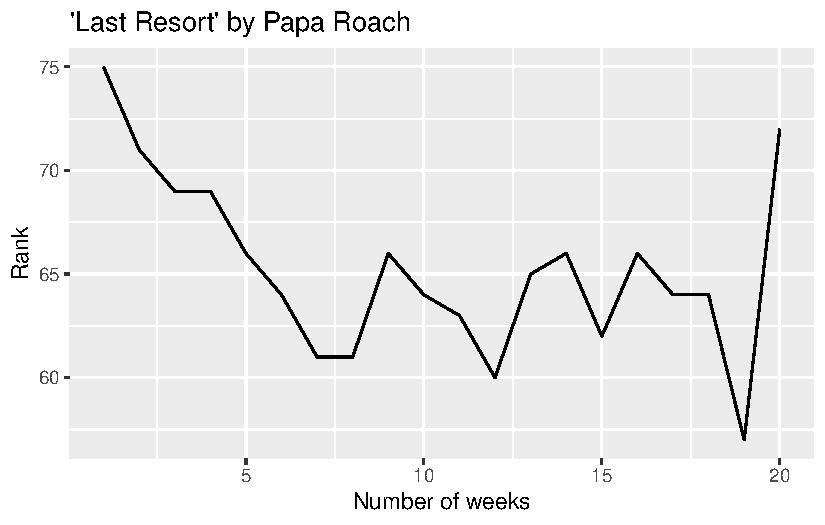
\includegraphics{_descr_stats_EN_files/figure-pdf/unnamed-chunk-16-1.pdf}

}

\end{figure}

\hypertarget{heutige-ziele}{%
\section*{Heutige Ziele}\label{heutige-ziele}}
\addcontentsline{toc}{section}{Heutige Ziele}

Today we will\ldots{}

\begin{itemize}
\tightlist
\item
  (re-)learn about measures of central tendency
\item
  (re-)learn about measures of dispersion
\item
  learn how to use the \texttt{summarise()} function from \texttt{dplyr}
\item
  learn how to produce summaries \texttt{.by} group
\end{itemize}

\hypertarget{lust-auf-mehr}{%
\subsection*{Lust auf mehr?}\label{lust-auf-mehr}}
\addcontentsline{toc}{subsection}{Lust auf mehr?}

Ch.4, Section 4.5 (Groups)
https://r4ds.hadley.nz/data-transform.html\#groups Wickham et al.
(o.~J.)

\hypertarget{einrichtung}{%
\section{Einrichtung}\label{einrichtung}}

\texttt{Session\ \textgreater{}\ Restart\ R} to start with a fresh
environment.

\begin{Shaded}
\begin{Highlighting}[]
\NormalTok{pacman}\SpecialCharTok{::}\FunctionTok{p\_load}\NormalTok{(tidyverse,}
\NormalTok{               here)}
\end{Highlighting}
\end{Shaded}

\begin{Shaded}
\begin{Highlighting}[]
\NormalTok{df\_flights }\OtherTok{\textless{}{-}} \FunctionTok{read\_csv}\NormalTok{(}\FunctionTok{here}\NormalTok{(}\StringTok{"daten"}\NormalTok{, }\StringTok{"flights.csv"}\NormalTok{))}
\end{Highlighting}
\end{Shaded}

\hypertarget{deskriptive-statistik}{%
\section{Deskriptive Statistik}\label{deskriptive-statistik}}

\begin{itemize}
\item
  descriptive statistics describe the central tendency, variability, and
  distribution of the data
\item
  sometimes called \texttt{summary} statistics, because it
  \emph{summarises} the observed data
\end{itemize}

\hypertarget{anzahl-der-werte-n}{%
\subsection{\texorpdfstring{Anzahl der Werte
(\(n\))}{Anzahl der Werte (n)}}\label{anzahl-der-werte-n}}

\begin{itemize}
\tightlist
\item
  important information when summarising data

  \begin{itemize}
  \tightlist
  \item
    when we have more data (higher \(n\)), we have more confidence in
    the conclusions we draw from our data because we have more evidence
  \item
    is also used to calculate some descriptive statistics
  \end{itemize}
\end{itemize}

\begin{Shaded}
\begin{Highlighting}[]
\NormalTok{values }\OtherTok{\textless{}{-}} \FunctionTok{c}\NormalTok{(}\DecValTok{3}\NormalTok{,}\DecValTok{1}\NormalTok{,}\DecValTok{2}\NormalTok{)}
\FunctionTok{length}\NormalTok{(values)}
\end{Highlighting}
\end{Shaded}

\begin{verbatim}
[1] 3
\end{verbatim}

\begin{center}\rule{0.5\linewidth}{0.5pt}\end{center}

\begin{tcolorbox}[enhanced jigsaw, left=2mm, breakable, colframe=quarto-callout-note-color-frame, toprule=.15mm, toptitle=1mm, titlerule=0mm, leftrule=.75mm, title=\textcolor{quarto-callout-note-color}{\faInfo}\hspace{0.5em}{\texttt{length()} versus \texttt{nrow()} and \texttt{n()}}, colbacktitle=quarto-callout-note-color!10!white, colback=white, coltitle=black, arc=.35mm, bottomtitle=1mm, opacityback=0, rightrule=.15mm, bottomrule=.15mm, opacitybacktitle=0.6]

\begin{itemize}
\tightlist
\item
  the function \texttt{length()} tells us how many (horizontal) values
  there are in an object

  \begin{itemize}
  \tightlist
  \item
    if that object is a data frame (instead of a vector like
    \texttt{values}), it tells us how many \emph{columns} we have
  \end{itemize}
\end{itemize}

\begin{Shaded}
\begin{Highlighting}[]
\FunctionTok{length}\NormalTok{(df\_flights)}
\end{Highlighting}
\end{Shaded}

\begin{verbatim}
[1] 19
\end{verbatim}

\begin{itemize}
\tightlist
\item
  to count the number of values (i.e., observations/rows) in a data
  frame we can use

  \begin{itemize}
  \tightlist
  \item
    \texttt{nrow()} (base R syntax), or
  \item
    \texttt{n()} (\texttt{dplyr} syntax), we'll see this later
  \end{itemize}
\end{itemize}

\begin{Shaded}
\begin{Highlighting}[]
\FunctionTok{nrow}\NormalTok{(df\_flights)}
\end{Highlighting}
\end{Shaded}

\begin{verbatim}
[1] 336776
\end{verbatim}

\end{tcolorbox}

\hypertarget{measures-of-central-tendency}{%
\subsection{Measures of central
tendency}\label{measures-of-central-tendency}}

\begin{itemize}
\tightlist
\item
  pretty much what we get for \emph{numeric} variables with the the
  \texttt{summary()} function
\end{itemize}

\begin{Shaded}
\begin{Highlighting}[]
\NormalTok{df\_flights }\SpecialCharTok{\%\textgreater{}\%} 
  \FunctionTok{select}\NormalTok{(air\_time, distance) }\SpecialCharTok{\%\textgreater{}\%} 
  \FunctionTok{summary}\NormalTok{() }\SpecialCharTok{\%\textgreater{}\%} 
\NormalTok{  knitr}\SpecialCharTok{::}\FunctionTok{kable}\NormalTok{() }\SpecialCharTok{\%\textgreater{}\%} 
\NormalTok{  kableExtra}\SpecialCharTok{::}\FunctionTok{kable\_styling}\NormalTok{(}\AttributeTok{font\_size =} \DecValTok{30}\NormalTok{)}
\end{Highlighting}
\end{Shaded}

\begin{table}
\centering\begingroup\fontsize{30}{32}\selectfont

\begin{tabular}{l|l|l}
\hline
  &    air\_time &    distance\\
\hline
 & Min.   : 20.0 & Min.   :  17\\
\hline
 & 1st Qu.: 82.0 & 1st Qu.: 502\\
\hline
 & Median :129.0 & Median : 872\\
\hline
 & Mean   :150.7 & Mean   :1040\\
\hline
 & 3rd Qu.:192.0 & 3rd Qu.:1389\\
\hline
 & Max.   :695.0 & Max.   :4983\\
\hline
 & NA's   :9430 & NA\\
\hline
\end{tabular}
\endgroup{}
\end{table}

\hypertarget{mean-mu}{%
\subsubsection{\texorpdfstring{Mean
(\(\mu\))}{Mean (\textbackslash mu)}}\label{mean-mu}}

\begin{itemize}
\tightlist
\item
  \texttt{mean} = Mittelwert, Durchschnitt
\item
  the sum of all values divided by the number of values
\end{itemize}

\[
\mu = \frac{Summe\;der\;Werte}
           {n}
\]

\begin{center}\rule{0.5\linewidth}{0.5pt}\end{center}

\begin{itemize}
\tightlist
\item
  we can easily compute the mean by hand when we have only a few values
\end{itemize}

\begin{Shaded}
\begin{Highlighting}[]
\NormalTok{(}\DecValTok{3}\SpecialCharTok{+}\DecValTok{1}\SpecialCharTok{+}\DecValTok{2}\NormalTok{)}\SpecialCharTok{/}\DecValTok{3}
\end{Highlighting}
\end{Shaded}

\begin{verbatim}
[1] 2
\end{verbatim}

\begin{itemize}
\tightlist
\item
  we can also save the values as a vector (a list of values of the same
  class)
\item
  and then use the function \texttt{mean()} to calculate their mean
\end{itemize}

\begin{Shaded}
\begin{Highlighting}[]
\NormalTok{values }\OtherTok{\textless{}{-}} \FunctionTok{c}\NormalTok{(}\DecValTok{3}\NormalTok{,}\DecValTok{1}\NormalTok{,}\DecValTok{2}\NormalTok{)}
\FunctionTok{mean}\NormalTok{(values)}
\end{Highlighting}
\end{Shaded}

\begin{verbatim}
[1] 2
\end{verbatim}

\begin{itemize}
\tightlist
\item
  or we can run the \texttt{mean()} function on a variable in a data
  frame

  \begin{itemize}
  \tightlist
  \item
    using the \texttt{\$} to indicate we want to select a column from a
    data frame
  \end{itemize}
\end{itemize}

\begin{Shaded}
\begin{Highlighting}[]
\FunctionTok{mean}\NormalTok{(df\_flights}\SpecialCharTok{$}\NormalTok{distance)}
\end{Highlighting}
\end{Shaded}

\begin{verbatim}
[1] 1039.913
\end{verbatim}

\begin{itemize}
\tightlist
\item
  \texttt{df\_flights\$distance} is similar to
  \texttt{df\_flights\ \%\textgreater{}\%\ select(distance)}
\end{itemize}

\hypertarget{median}{%
\subsubsection{Median}\label{median}}

\begin{itemize}
\tightlist
\item
  \texttt{median} = Median, mediane Wert; the value in the middle of the
  dataset
\item
  if you line up all your values in ascending (or descending) order, the
  middle value is the median

  \begin{itemize}
  \tightlist
  \item
    e.g., if you have 5 values, the 3rd value is the median
  \item
    if you have 6 values, the mean of the 3rd and 4th values are the
    median
  \end{itemize}
\item
  50\% of the data lie below this value, 50\% above it
\end{itemize}

\begin{Shaded}
\begin{Highlighting}[]
\FunctionTok{median}\NormalTok{(df\_flights}\SpecialCharTok{$}\NormalTok{distance)}
\end{Highlighting}
\end{Shaded}

\begin{verbatim}
[1] 872
\end{verbatim}

\hypertarget{mode}{%
\subsubsection{Mode}\label{mode}}

\begin{itemize}
\tightlist
\item
  \texttt{mode} = Modalwert; the value that occurs the most in a data
  set
\item
  there's no R function to determine the \texttt{mode}, but we can
  visualise it with a histogram
\end{itemize}

\begin{Shaded}
\begin{Highlighting}[]
\NormalTok{df\_flights }\SpecialCharTok{\%\textgreater{}\%} 
  \FunctionTok{ggplot}\NormalTok{(}\FunctionTok{aes}\NormalTok{(}\AttributeTok{x =}\NormalTok{ distance)) }\SpecialCharTok{+}
  \FunctionTok{geom\_histogram}\NormalTok{() }\SpecialCharTok{+}
  \FunctionTok{theme\_minimal}\NormalTok{() }
\end{Highlighting}
\end{Shaded}

\begin{figure}[H]

{\centering 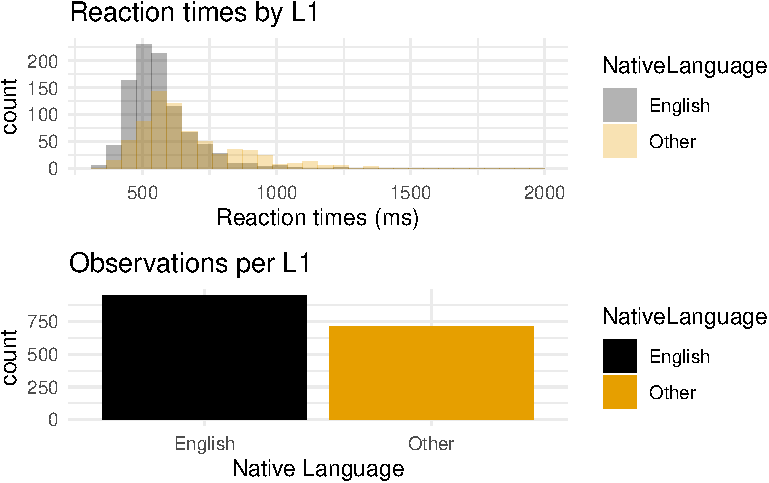
\includegraphics{_descr_stats_EN_files/figure-pdf/unnamed-chunk-27-1.pdf}

}

\end{figure}

\hypertarget{measures-of-dispersion}{%
\subsection{Measures of dispersion}\label{measures-of-dispersion}}

\begin{itemize}
\tightlist
\item
  measures of central tendency describe the middle of the data (usually)
\item
  measures of dispersion describe the spread of data points
\end{itemize}

\hypertarget{range}{%
\subsubsection{Range}\label{range}}

\begin{itemize}
\tightlist
\item
  \texttt{range} = Wertebereich

  \begin{itemize}
  \tightlist
  \item
    can refer to the highest and lowest values, or
  \item
    the difference between highest and lowest value
  \end{itemize}
\end{itemize}

\begin{center}\rule{0.5\linewidth}{0.5pt}\end{center}

\begin{itemize}
\tightlist
\item
  \texttt{max()} and \texttt{min()} print the highest and lowest values
\end{itemize}

\begin{Shaded}
\begin{Highlighting}[]
\FunctionTok{max}\NormalTok{(values)}
\end{Highlighting}
\end{Shaded}

\begin{verbatim}
[1] 3
\end{verbatim}

\begin{Shaded}
\begin{Highlighting}[]
\FunctionTok{min}\NormalTok{(values)}
\end{Highlighting}
\end{Shaded}

\begin{verbatim}
[1] 1
\end{verbatim}

\begin{itemize}
\tightlist
\item
  \texttt{range()} prints the lowest and highest values
\end{itemize}

\begin{Shaded}
\begin{Highlighting}[]
\FunctionTok{range}\NormalTok{(values)}
\end{Highlighting}
\end{Shaded}

\begin{verbatim}
[1] 1 3
\end{verbatim}

\begin{itemize}
\tightlist
\item
  we can calculate the difference between these values:
\end{itemize}

\begin{Shaded}
\begin{Highlighting}[]
\FunctionTok{max}\NormalTok{(values) }\SpecialCharTok{{-}} \FunctionTok{min}\NormalTok{(values)}
\end{Highlighting}
\end{Shaded}

\begin{verbatim}
[1] 2
\end{verbatim}

\hypertarget{standard-deviation-sd-or-sigma}{%
\subsubsection{\texorpdfstring{Standard deviation (\texttt{sd} or
\(\sigma\))}{Standard deviation (sd or \textbackslash sigma)}}\label{standard-deviation-sd-or-sigma}}

\begin{itemize}
\item
  a measure of how dispersed that data is \emph{in relation to the mean}

  \begin{itemize}
  \tightlist
  \item
    low standard deviation means data are clustered around the mean
    (i.e., there is less spread)
  \item
    high standard deviation means data are more spread out
  \end{itemize}
\item
  standard deviation is very often reported whenever mean is reported
\item
  to calculate \texttt{sd}

  \begin{itemize}
  \tightlist
  \item
    the square root (\(\sqrt{}\)) of the sum of squared value deviations
    from the mean (\((x - \mu)^2\)) divided by the number of
    observations minus 1 (\(n-1\))
  \end{itemize}
\end{itemize}

\begin{Shaded}
\begin{Highlighting}[]
\FunctionTok{sd}\NormalTok{(values)}
\end{Highlighting}
\end{Shaded}

\begin{verbatim}
[1] 1
\end{verbatim}

\begin{center}\rule{0.5\linewidth}{0.5pt}\end{center}

\begin{itemize}
\tightlist
\item
  our values (\(x\)) are:
\end{itemize}

\begin{Shaded}
\begin{Highlighting}[]
\NormalTok{values}
\end{Highlighting}
\end{Shaded}

\begin{verbatim}
[1] 3 1 2
\end{verbatim}

\begin{itemize}
\tightlist
\item
  the mean (\(\mu\)) is:
\end{itemize}

\begin{Shaded}
\begin{Highlighting}[]
\FunctionTok{mean}\NormalTok{(values)}
\end{Highlighting}
\end{Shaded}

\begin{verbatim}
[1] 2
\end{verbatim}

\begin{itemize}
\tightlist
\item
  the number of values (\(n\)) is:
\end{itemize}

\begin{Shaded}
\begin{Highlighting}[]
\FunctionTok{length}\NormalTok{(values)}
\end{Highlighting}
\end{Shaded}

\begin{verbatim}
[1] 3
\end{verbatim}

\begin{itemize}
\tightlist
\item
  the standard deviation (\(\sigma\)) is:
\end{itemize}

\begin{Shaded}
\begin{Highlighting}[]
\FunctionTok{sd}\NormalTok{(values)}
\end{Highlighting}
\end{Shaded}

\begin{verbatim}
[1] 1
\end{verbatim}

\begin{align}

\sigma & = \sqrt{\frac{(x_1-\mu)^2 + (x_2-\mu)^2 + (x_3-\mu)^2}{N-1}}
\\
& = \sqrt{\frac{(3-\mu)^2 + (1-\mu)^2 + (2-\mu)^2}{N-1}}
\\
& = \sqrt{\frac{(3-2)^2 + (1-2)^2 + (2-2)^2}{3-1}}
\\
& = \sqrt{\frac{(1)^2 + (-1)^2 + (0)^2}{2}}
\\
& = \sqrt{\frac{1 + 1 + 0}{2}}
\\
& = \sqrt{\frac{2}{2}} = \sqrt{1} = 1

\end{align}

\begin{center}\rule{0.5\linewidth}{0.5pt}\end{center}

\begin{itemize}
\tightlist
\item
  how is the standard deviation helpful?

  \begin{itemize}
  \tightlist
  \item
    it gives us a measure of how ``tight'' the observed values are to
    the mean
  \end{itemize}
\item
  different datasets can have the same mean, for example:
\end{itemize}

\begin{Shaded}
\begin{Highlighting}[]
\NormalTok{values2 }\OtherTok{\textless{}{-}} \FunctionTok{c}\NormalTok{(}\DecValTok{55}\NormalTok{,}\DecValTok{55}\NormalTok{,}\DecValTok{55}\NormalTok{,}\DecValTok{55}\NormalTok{,}\DecValTok{55}\NormalTok{,}\DecValTok{57}\NormalTok{,}\DecValTok{57}\NormalTok{,}\DecValTok{57}\NormalTok{,}\DecValTok{57}\NormalTok{,}\DecValTok{57}\NormalTok{)}
\NormalTok{values3 }\OtherTok{\textless{}{-}} \FunctionTok{c}\NormalTok{(}\DecValTok{1}\NormalTok{,}\DecValTok{1}\NormalTok{,}\DecValTok{1}\NormalTok{,}\DecValTok{1}\NormalTok{,}\DecValTok{100}\NormalTok{,}\DecValTok{100}\NormalTok{,}\DecValTok{100}\NormalTok{,}\DecValTok{100}\NormalTok{,}\DecValTok{100}\NormalTok{)}
\end{Highlighting}
\end{Shaded}

\begin{Shaded}
\begin{Highlighting}[]
\FunctionTok{mean}\NormalTok{(values2)}
\end{Highlighting}
\end{Shaded}

\begin{verbatim}
[1] 56
\end{verbatim}

\begin{Shaded}
\begin{Highlighting}[]
\FunctionTok{mean}\NormalTok{(values3)}
\end{Highlighting}
\end{Shaded}

\begin{verbatim}
[1] 56
\end{verbatim}

\begin{itemize}
\tightlist
\item
  \texttt{values2} and \texttt{values3} have the same mean

  \begin{itemize}
  \tightlist
  \item
    if we only calculated the mean, we might conclude the data are
    similar
  \end{itemize}
\item
  but their standard deviations will differ, because their respective
  observed values all differ in how far they deviate from the mean
\item
  which vector do you think will have the \emph{smallest} standard
  deviation? Why?
\end{itemize}

\begin{Shaded}
\begin{Highlighting}[]
\FunctionTok{sd}\NormalTok{(values2)}
\end{Highlighting}
\end{Shaded}

\begin{verbatim}
[1] 1.054093
\end{verbatim}

\begin{Shaded}
\begin{Highlighting}[]
\FunctionTok{sd}\NormalTok{(values3)}
\end{Highlighting}
\end{Shaded}

\begin{verbatim}
[1] 52.17758
\end{verbatim}

\begin{center}\rule{0.5\linewidth}{0.5pt}\end{center}

\begin{tcolorbox}[enhanced jigsaw, left=2mm, breakable, colframe=quarto-callout-note-color-frame, toprule=.15mm, toptitle=1mm, titlerule=0mm, leftrule=.75mm, title=\textcolor{quarto-callout-note-color}{\faInfo}\hspace{0.5em}{Calculating standard deviation}, colbacktitle=quarto-callout-note-color!10!white, colback=white, coltitle=black, arc=.35mm, bottomtitle=1mm, opacityback=0, rightrule=.15mm, bottomrule=.15mm, opacitybacktitle=0.6]

\begin{itemize}
\tightlist
\item
  first, calculate the deviation of each value from the mean

  \begin{itemize}
  \tightlist
  \item
    and square this value
  \end{itemize}
\item
  add up all these squared deviation values

  \begin{itemize}
  \tightlist
  \item
    divide by the number of observations \emph{minue one} (\(n-1\))
  \end{itemize}
\item
  this is now the \emph{variance}, to get the population standard
  deviation, compute the square root of this value
\end{itemize}

\begin{align}

\sigma & = \sqrt\frac{(56-1)^2 + (56-1)^2 + (56-1)^2 + (56-1)^2 + (56-100)^2 +
        (56-100)^2 + (56-100)^2 + (56-100)^2 + (56-100)^2 + (56-100)^2}{n-1}
\\
& = \sqrt{\frac{3025 + 3025 + 3025 + 3025 + 1936 + 1936 + 1936 + 1936 + 1936}{9-1}}
\\
& = \sqrt{\frac{21780}{8}}
\\
& = \sqrt{2722.5}
\\
& = 52.17758

\end{align}

\begin{itemize}
\item
  since we divide by the number of observations (minus 1), if we have
  \emph{more} observations (and therefore divide by a larger number),
  the standard deviation will be smaller (because when we divide by a
  large number the product is much smaller)
\item
  consider: if we divide 100 by the number 2, the result is 50. If we
  divide 100 by a larger number, like 50, then the result (2) is smaller
\end{itemize}

\end{tcolorbox}

\hypertarget{dplyrsummarise}{%
\section{\texorpdfstring{\texttt{dplyr::summarise}}{dplyr::summarise}}\label{dplyrsummarise}}

\begin{itemize}
\tightlist
\item
  computes summaries of data

  \begin{itemize}
  \tightlist
  \item
    but we have to tell it \emph{what} to compute, and for which
    variable(s)
  \end{itemize}
\end{itemize}

\begin{Shaded}
\begin{Highlighting}[]
\NormalTok{df\_flights }\SpecialCharTok{\%\textgreater{}\%} 
  \FunctionTok{summarise}\NormalTok{(}\AttributeTok{N =} \FunctionTok{n}\NormalTok{())}
\end{Highlighting}
\end{Shaded}

\begin{verbatim}
# A tibble: 1 x 1
       N
   <int>
1 336776
\end{verbatim}

\begin{center}\rule{0.5\linewidth}{0.5pt}\end{center}

\begin{itemize}
\tightlist
\item
  we can also run multiple computations at once
\end{itemize}

\begin{Shaded}
\begin{Highlighting}[]
\NormalTok{df\_flights }\SpecialCharTok{\%\textgreater{}\%} 
  \FunctionTok{summarise}\NormalTok{(}\AttributeTok{mean\_distance =} \FunctionTok{mean}\NormalTok{(distance, }\AttributeTok{na.rm=}\NormalTok{T),}
            \AttributeTok{sd\_distance =} \FunctionTok{sd}\NormalTok{(distance, }\AttributeTok{na.rm =}\NormalTok{ T),}
            \AttributeTok{N =} \FunctionTok{n}\NormalTok{()) }\SpecialCharTok{\%\textgreater{}\%} 
\NormalTok{  knitr}\SpecialCharTok{::}\FunctionTok{kable}\NormalTok{() }\SpecialCharTok{\%\textgreater{}\%} 
\NormalTok{  kableExtra}\SpecialCharTok{::}\FunctionTok{kable\_styling}\NormalTok{()}
\end{Highlighting}
\end{Shaded}

\begin{table}
\centering
\begin{tabular}{r|r|r}
\hline
mean\_distance & sd\_distance & N\\
\hline
1039.913 & 733.233 & 336776\\
\hline
\end{tabular}
\end{table}

\begin{center}\rule{0.5\linewidth}{0.5pt}\end{center}

\begin{itemize}
\tightlist
\item
  and we can specify calculations
\end{itemize}

\begin{Shaded}
\begin{Highlighting}[]
\NormalTok{df\_flights }\SpecialCharTok{\%\textgreater{}\%} 
  \FunctionTok{summarise}\NormalTok{(}\AttributeTok{range\_distance =} \FunctionTok{max}\NormalTok{(distance) }\SpecialCharTok{{-}} \FunctionTok{min}\NormalTok{(distance))}
\end{Highlighting}
\end{Shaded}

\begin{verbatim}
# A tibble: 1 x 1
  range_distance
           <dbl>
1           4966
\end{verbatim}

\hypertarget{missing-values}{%
\subsection{Missing values}\label{missing-values}}

\begin{itemize}
\tightlist
\item
  some calculations aren't possible if there are missing values

  \begin{itemize}
  \tightlist
  \item
    the variable \texttt{air\_time} has some missing values
  \end{itemize}
\end{itemize}

\begin{Shaded}
\begin{Highlighting}[]
\NormalTok{df\_flights }\SpecialCharTok{\%\textgreater{}\%} 
  \FunctionTok{select}\NormalTok{(air\_time, distance) }\SpecialCharTok{\%\textgreater{}\%} 
  \FunctionTok{summary}\NormalTok{()}
\end{Highlighting}
\end{Shaded}

\begin{verbatim}
    air_time        distance   
 Min.   : 20.0   Min.   :  17  
 1st Qu.: 82.0   1st Qu.: 502  
 Median :129.0   Median : 872  
 Mean   :150.7   Mean   :1040  
 3rd Qu.:192.0   3rd Qu.:1389  
 Max.   :695.0   Max.   :4983  
 NA's   :9430                  
\end{verbatim}

\begin{Shaded}
\begin{Highlighting}[]
\NormalTok{df\_flights }\SpecialCharTok{\%\textgreater{}\%} 
  \FunctionTok{summarise}\NormalTok{(}\AttributeTok{mean\_air\_time =} \FunctionTok{mean}\NormalTok{(air\_time))}
\end{Highlighting}
\end{Shaded}

\begin{verbatim}
# A tibble: 1 x 1
  mean_air_time
          <dbl>
1            NA
\end{verbatim}

\begin{center}\rule{0.5\linewidth}{0.5pt}\end{center}

\begin{itemize}
\tightlist
\item
  when working with real data, how we deal with missing values is not
  trivial

  \begin{itemize}
  \tightlist
  \item
    e.g., we might want to convert all \texttt{NA} values to \texttt{0}
    if we want them to contribute to the calculation of the
    \texttt{mean}
  \item
    but more often than not, we want to just remove them (as we have
    often already done)
  \end{itemize}
\item
  we can easily do this with the \texttt{dplyr} verb \texttt{drop\_na()}
\end{itemize}

\begin{Shaded}
\begin{Highlighting}[]
\NormalTok{df\_flights }\SpecialCharTok{\%\textgreater{}\%} 
  \FunctionTok{drop\_na}\NormalTok{() }\SpecialCharTok{\%\textgreater{}\%} 
  \FunctionTok{summarise}\NormalTok{(}\AttributeTok{mean =} \FunctionTok{mean}\NormalTok{(air\_time))}
\end{Highlighting}
\end{Shaded}

\begin{verbatim}
# A tibble: 1 x 1
   mean
  <dbl>
1  151.
\end{verbatim}

\hypertarget{grouping-variables}{%
\section{Grouping variables}\label{grouping-variables}}

\begin{itemize}
\tightlist
\item
  we don't always just want to know the summary statistics for an entire
  dataset, however

  \begin{itemize}
  \tightlist
  \item
    we usually want to \emph{compare} certain groups (e.g., comparing
    \texttt{air\_time} between airline \texttt{carriers})
  \end{itemize}
\end{itemize}

\hypertarget{by}{%
\subsection{\texorpdfstring{\texttt{.by\ =}}{.by =}}\label{by}}

\begin{itemize}
\tightlist
\item
  the brand new \texttt{.by\ =} argument in \texttt{summarise()}
  computes our calculations on grouped subsets of the data (only a few
  months old!)

  \begin{itemize}
  \tightlist
  \item
    it takes a \texttt{variable} (i.e., column name), and groups by the
    levels of this variable
  \end{itemize}
\end{itemize}

\begin{center}\rule{0.5\linewidth}{0.5pt}\end{center}

\begin{Shaded}
\begin{Highlighting}[]
\NormalTok{df\_flights }\SpecialCharTok{\%\textgreater{}\%} 
  \FunctionTok{drop\_na}\NormalTok{() }\SpecialCharTok{\%\textgreater{}\%} 
  \FunctionTok{summarise}\NormalTok{(}\AttributeTok{mean\_air\_time =} \FunctionTok{mean}\NormalTok{(air\_time),}
            \AttributeTok{mean\_distance =} \FunctionTok{mean}\NormalTok{(distance),}
            \AttributeTok{N =} \FunctionTok{n}\NormalTok{(),}
            \AttributeTok{.by =}\NormalTok{ month) }\SpecialCharTok{\%\textgreater{}\%} 
  \FunctionTok{arrange}\NormalTok{(mean\_air\_time)}
\end{Highlighting}
\end{Shaded}

\begin{verbatim}
# A tibble: 12 x 4
   month mean_air_time mean_distance     N
   <dbl>         <dbl>         <dbl> <int>
 1     9          143.         1049. 27010
 2     5          146.         1049. 28128
 3     7          147.         1070. 28293
 4     8          148.         1069. 28756
 5    10          149.         1042. 28618
 6     3          149.         1023. 27902
 7     6          150.         1074. 27075
 8     2          151.         1008. 23611
 9     4          153.         1048. 27564
10     1          154.         1014. 26398
11    11          155.         1052. 26971
12    12          163.         1076. 27020
\end{verbatim}

\hypertarget{group-by-multiple-variables}{%
\subsection{Group by multiple
variables}\label{group-by-multiple-variables}}

\begin{itemize}
\tightlist
\item
  we can also group by multiple variables

  \begin{itemize}
  \tightlist
  \item
    for this we need \texttt{concatenate} (\texttt{c()})
  \end{itemize}
\item
  we'll filter to only have a couple of carriers, just so our output
  isn't too long
\end{itemize}

\begin{center}\rule{0.5\linewidth}{0.5pt}\end{center}

\begin{Shaded}
\begin{Highlighting}[numbers=left,,]
\NormalTok{df\_flights }\SpecialCharTok{\%\textgreater{}\%} 
  \FunctionTok{drop\_na}\NormalTok{() }\SpecialCharTok{\%\textgreater{}\%}
  \FunctionTok{filter}\NormalTok{(carrier }\SpecialCharTok{\%in\%} \FunctionTok{c}\NormalTok{(}\StringTok{"UA"}\NormalTok{, }\StringTok{"AA"}\NormalTok{)) }\SpecialCharTok{\%\textgreater{}\%} 
  \FunctionTok{summarise}\NormalTok{(}\AttributeTok{mean\_air\_time =} \FunctionTok{mean}\NormalTok{(air\_time),}
            \AttributeTok{mean\_distance =} \FunctionTok{mean}\NormalTok{(distance),}
            \AttributeTok{N =} \FunctionTok{n}\NormalTok{(),}
            \AttributeTok{.by =} \FunctionTok{c}\NormalTok{(month, carrier)) }\SpecialCharTok{\%\textgreater{}\%} 
  \FunctionTok{arrange}\NormalTok{(month, carrier) }\SpecialCharTok{\%\textgreater{}\%} 
\NormalTok{  knitr}\SpecialCharTok{::}\FunctionTok{kable}\NormalTok{() }\SpecialCharTok{\%\textgreater{}\%} 
\NormalTok{  kableExtra}\SpecialCharTok{::}\FunctionTok{kable\_styling}\NormalTok{(}\AttributeTok{font\_size =} \DecValTok{20}\NormalTok{)}
\end{Highlighting}
\end{Shaded}

\begin{table}
\centering\begingroup\fontsize{20}{22}\selectfont

\begin{tabular}{r|l|r|r|r}
\hline
month & carrier & mean\_air\_time & mean\_distance & N\\
\hline
1 & AA & 199.5433 & 1353.099 & 2724\\
\hline
1 & UA & 213.7022 & 1463.894 & 4590\\
\hline
2 & AA & 197.9195 & 1352.686 & 2399\\
\hline
2 & UA & 207.4393 & 1437.190 & 4157\\
\hline
3 & AA & 192.3532 & 1349.525 & 2741\\
\hline
3 & UA & 204.7959 & 1454.933 & 4909\\
\hline
4 & AA & 192.9615 & 1343.950 & 2649\\
\hline
4 & UA & 212.0633 & 1504.828 & 4978\\
\hline
5 & AA & 183.4554 & 1341.822 & 2749\\
\hline
5 & UA & 209.1620 & 1559.828 & 4890\\
\hline
6 & AA & 183.4868 & 1338.606 & 2683\\
\hline
6 & UA & 213.0440 & 1580.517 & 4885\\
\hline
7 & AA & 178.3669 & 1328.671 & 2769\\
\hline
7 & UA & 207.8638 & 1581.408 & 4971\\
\hline
8 & AA & 179.4030 & 1326.186 & 2819\\
\hline
8 & UA & 212.0912 & 1593.323 & 5085\\
\hline
9 & AA & 179.3695 & 1344.793 & 2568\\
\hline
9 & UA & 208.0990 & 1571.911 & 4636\\
\hline
10 & AA & 186.8477 & 1337.230 & 2699\\
\hline
10 & UA & 210.3654 & 1528.576 & 5035\\
\hline
11 & AA & 193.3208 & 1344.323 & 2550\\
\hline
11 & UA & 218.2343 & 1534.453 & 4827\\
\hline
12 & AA & 200.7724 & 1361.288 & 2597\\
\hline
12 & UA & 224.2924 & 1546.725 & 4819\\
\hline
\end{tabular}
\endgroup{}
\end{table}

\begin{center}\rule{0.5\linewidth}{0.5pt}\end{center}

\begin{tcolorbox}[enhanced jigsaw, left=2mm, breakable, colframe=quarto-callout-note-color-frame, toprule=.15mm, toptitle=1mm, titlerule=0mm, leftrule=.75mm, title=\textcolor{quarto-callout-note-color}{\faInfo}\hspace{0.5em}{\texttt{group\_by()}}, colbacktitle=quarto-callout-note-color!10!white, colback=white, coltitle=black, arc=.35mm, bottomtitle=1mm, opacityback=0, rightrule=.15mm, bottomrule=.15mm, opacitybacktitle=0.6]

\begin{itemize}
\tightlist
\item
  before \texttt{.by()}, we used to use the \texttt{dplyr} verb
  \texttt{group\_by()} and \texttt{ungroup()}

  \begin{itemize}
  \tightlist
  \item
    I prefer the new \texttt{.by}, because it keeps the grouping local
    (no need to \texttt{ungroup()})
  \item
    keep this in mind, you might see \texttt{group\_by()} in the wild
  \end{itemize}
\end{itemize}

\begin{Shaded}
\begin{Highlighting}[numbers=left,,]
\NormalTok{df\_flights }\SpecialCharTok{\%\textgreater{}\%} 
  \FunctionTok{drop\_na}\NormalTok{() }\SpecialCharTok{\%\textgreater{}\%}
  \FunctionTok{filter}\NormalTok{(carrier }\SpecialCharTok{\%in\%} \FunctionTok{c}\NormalTok{(}\StringTok{"UA"}\NormalTok{, }\StringTok{"AA"}\NormalTok{)) }\SpecialCharTok{\%\textgreater{}\%} 
  \FunctionTok{group\_by}\NormalTok{(month, carrier) }\SpecialCharTok{\%\textgreater{}\%} 
  \FunctionTok{summarise}\NormalTok{(}\AttributeTok{mean\_air\_time =} \FunctionTok{mean}\NormalTok{(air\_time),}
            \AttributeTok{mean\_distance =} \FunctionTok{mean}\NormalTok{(distance),}
            \AttributeTok{N =} \FunctionTok{n}\NormalTok{()) }\SpecialCharTok{\%\textgreater{}\%} 
  \FunctionTok{ungroup}\NormalTok{() }\SpecialCharTok{\%\textgreater{}\%} 
  \FunctionTok{arrange}\NormalTok{(month, carrier) }\SpecialCharTok{\%\textgreater{}\%} 
  \FunctionTok{head}\NormalTok{(}\AttributeTok{n =} \DecValTok{10}\NormalTok{) }\SpecialCharTok{\%\textgreater{}\%} 
\NormalTok{  knitr}\SpecialCharTok{::}\FunctionTok{kable}\NormalTok{() }\SpecialCharTok{\%\textgreater{}\%} 
\NormalTok{  kableExtra}\SpecialCharTok{::}\FunctionTok{kable\_styling}\NormalTok{(}\AttributeTok{font\_size =} \DecValTok{20}\NormalTok{) }
\end{Highlighting}
\end{Shaded}

\begin{table}
\centering\begingroup\fontsize{20}{22}\selectfont

\begin{tabular}{r|l|r|r|r}
\hline
month & carrier & mean\_air\_time & mean\_distance & N\\
\hline
1 & AA & 199.5433 & 1353.099 & 2724\\
\hline
1 & UA & 213.7022 & 1463.894 & 4590\\
\hline
2 & AA & 197.9195 & 1352.686 & 2399\\
\hline
2 & UA & 207.4393 & 1437.190 & 4157\\
\hline
3 & AA & 192.3532 & 1349.525 & 2741\\
\hline
3 & UA & 204.7959 & 1454.933 & 4909\\
\hline
4 & AA & 192.9615 & 1343.950 & 2649\\
\hline
4 & UA & 212.0633 & 1504.828 & 4978\\
\hline
5 & AA & 183.4554 & 1341.822 & 2749\\
\hline
5 & UA & 209.1620 & 1559.828 & 4890\\
\hline
\end{tabular}
\endgroup{}
\end{table}

\end{tcolorbox}

\hypertarget{anscombes-quartet}{%
\section{Anscombe's Quartet}\label{anscombes-quartet}}

\begin{itemize}
\tightlist
\item
  Francis Anscombe constructed 4 datasets in 1973 to illustrate the
  importance of visualising data before analysing it and building a
  model

  \begin{itemize}
  \tightlist
  \item
    these four plots represent 4 datasets that all have nearly identical
    mean and standard deviation, but very different distributions
  \end{itemize}
\end{itemize}

\hypertarget{tbl-anscombe}{}
\begin{table}
\caption{\label{tbl-anscombe}Summary stats of Anscombe's quratet datasets }\tabularnewline

\centering\begingroup\fontsize{20}{22}\selectfont

\begin{tabular}{l|r|r|r|r|r|r|r}
\hline
grp & mean\_x & mean\_y & min\_x & min\_y & max\_x & max\_y & crrltn\\
\hline
Group 1 & 9 & 7.500909 & 4 & 4.26 & 14 & 10.84 & 0.8164205\\
\hline
Group 2 & 9 & 7.500909 & 4 & 3.10 & 14 & 9.26 & 0.8162365\\
\hline
Group 3 & 9 & 7.500000 & 4 & 5.39 & 14 & 12.74 & 0.8162867\\
\hline
Group 4 & 9 & 7.500909 & 8 & 5.25 & 19 & 12.50 & 0.8165214\\
\hline
\end{tabular}
\endgroup{}
\end{table}

\begin{center}\rule{0.5\linewidth}{0.5pt}\end{center}

\begin{figure}

{\centering 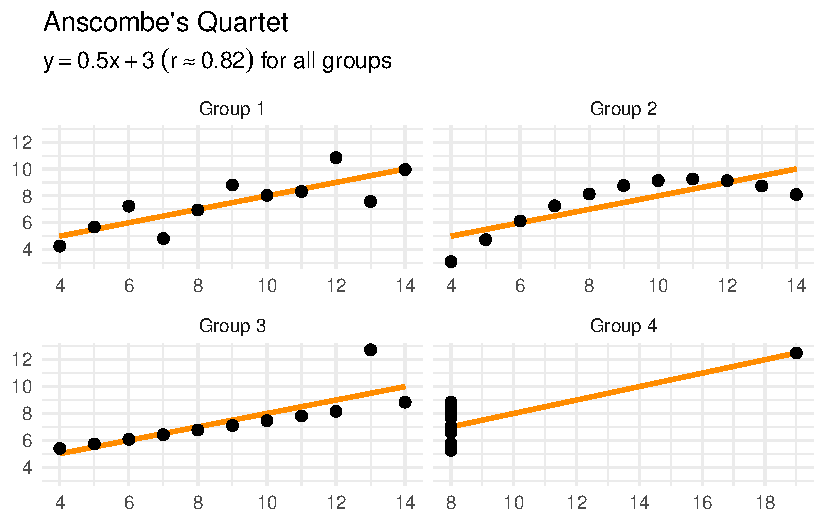
\includegraphics{_descr_stats_EN_files/figure-pdf/fig-anscombe-1.pdf}

}

\caption{\label{fig-anscombe}Plots of Anscombe's quratet distributions}

\end{figure}

\hypertarget{datasaurrus}{%
\subsection{DatasaurRus}\label{datasaurrus}}

\begin{itemize}
\tightlist
\item
  the datasaurRs package contains some more datasets that have similar
  mean and sd, but different distributions
\end{itemize}

\begin{Shaded}
\begin{Highlighting}[]
\NormalTok{pacman}\SpecialCharTok{::}\FunctionTok{p\_load}\NormalTok{(}\StringTok{"datasauRus"}\NormalTok{)}
\end{Highlighting}
\end{Shaded}

\begin{Shaded}
\begin{Highlighting}[]
\NormalTok{datasaurus\_dozen }\SpecialCharTok{\%\textgreater{}\%} 
    \FunctionTok{group\_by}\NormalTok{(dataset) }\SpecialCharTok{\%\textgreater{}\%} 
    \FunctionTok{summarize}\NormalTok{(}
      \AttributeTok{mean\_x    =} \FunctionTok{mean}\NormalTok{(x),}
      \AttributeTok{mean\_y    =} \FunctionTok{mean}\NormalTok{(y),}
      \AttributeTok{std\_dev\_x =} \FunctionTok{sd}\NormalTok{(x),}
      \AttributeTok{std\_dev\_y =} \FunctionTok{sd}\NormalTok{(y),}
      \AttributeTok{corr\_x\_y  =} \FunctionTok{cor}\NormalTok{(x, y)}
\NormalTok{    ) }\SpecialCharTok{\%\textgreater{}\%} 
\NormalTok{  knitr}\SpecialCharTok{::}\FunctionTok{kable}\NormalTok{() }\SpecialCharTok{\%\textgreater{}\%} 
\NormalTok{  kableExtra}\SpecialCharTok{::}\FunctionTok{kable\_styling}\NormalTok{(}\AttributeTok{font\_size =} \DecValTok{20}\NormalTok{)}
\end{Highlighting}
\end{Shaded}

\hypertarget{tbl-datasauRus}{}
\begin{table}
\caption{\label{tbl-datasauRus}Summary stats of datasauRus datasets }\tabularnewline

\centering\begingroup\fontsize{20}{22}\selectfont

\begin{tabular}{l|r|r|r|r|r}
\hline
dataset & mean\_x & mean\_y & std\_dev\_x & std\_dev\_y & corr\_x\_y\\
\hline
away & 54.26610 & 47.83472 & 16.76983 & 26.93974 & -0.0641284\\
\hline
bullseye & 54.26873 & 47.83082 & 16.76924 & 26.93573 & -0.0685864\\
\hline
circle & 54.26732 & 47.83772 & 16.76001 & 26.93004 & -0.0683434\\
\hline
dino & 54.26327 & 47.83225 & 16.76514 & 26.93540 & -0.0644719\\
\hline
dots & 54.26030 & 47.83983 & 16.76774 & 26.93019 & -0.0603414\\
\hline
h\_lines & 54.26144 & 47.83025 & 16.76590 & 26.93988 & -0.0617148\\
\hline
high\_lines & 54.26881 & 47.83545 & 16.76670 & 26.94000 & -0.0685042\\
\hline
slant\_down & 54.26785 & 47.83590 & 16.76676 & 26.93610 & -0.0689797\\
\hline
slant\_up & 54.26588 & 47.83150 & 16.76885 & 26.93861 & -0.0686092\\
\hline
star & 54.26734 & 47.83955 & 16.76896 & 26.93027 & -0.0629611\\
\hline
v\_lines & 54.26993 & 47.83699 & 16.76996 & 26.93768 & -0.0694456\\
\hline
wide\_lines & 54.26692 & 47.83160 & 16.77000 & 26.93790 & -0.0665752\\
\hline
x\_shape & 54.26015 & 47.83972 & 16.76996 & 26.93000 & -0.0655833\\
\hline
\end{tabular}
\endgroup{}
\end{table}

\begin{center}\rule{0.5\linewidth}{0.5pt}\end{center}

\begin{itemize}
\tightlist
\item
  if we plot the datasets, they all look very different!
\end{itemize}

\begin{figure}

{\centering 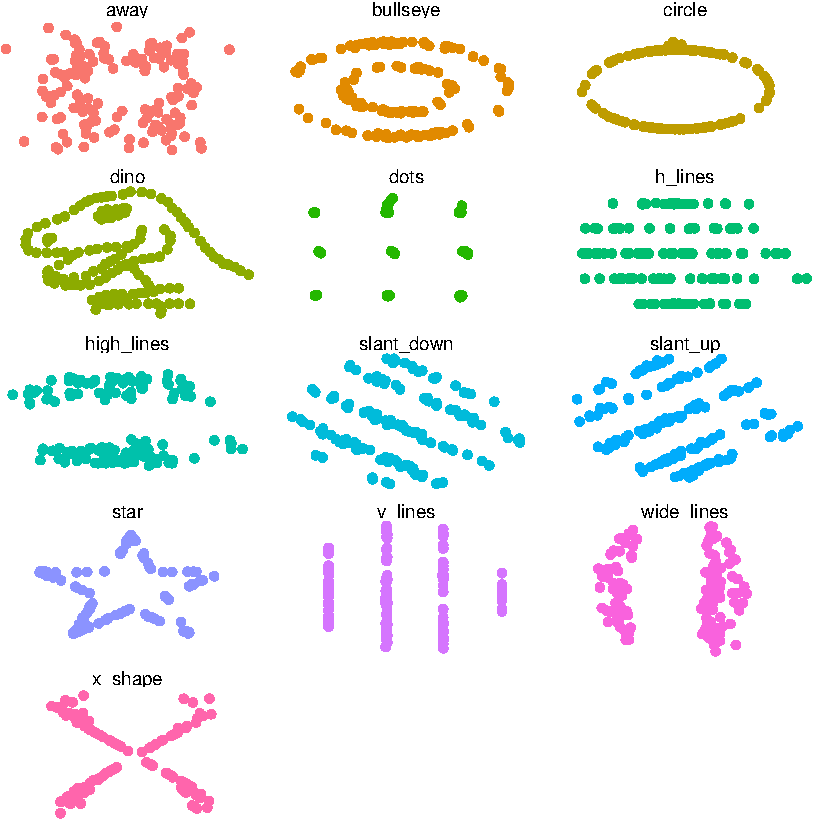
\includegraphics[width=0.5\textwidth,height=\textheight]{_descr_stats_EN_files/figure-pdf/fig-datasauRus-1.pdf}

}

\caption{\label{fig-datasauRus}Plots of datasauRus dataset
distributions}

\end{figure}

\hypertarget{aufgaben}{%
\section{Aufgaben}\label{aufgaben}}

\begin{enumerate}
\def\labelenumi{\arabic{enumi}.}
\tightlist
\item
  Calculate the standard deviation of the values
  \texttt{152,\ 19,\ 1398,\ 67,\ 2111} without using the function
  \texttt{sd()}

  \begin{itemize}
  \tightlist
  \item
    show your work. The following R syntax might be useful (depending on
    how you decide to do it):

    \begin{itemize}
    \tightlist
    \item
      \texttt{c()}
    \item
      \texttt{mean()}
    \item
      \texttt{x\^{}2} calculates the square of a value (here,
      \texttt{x})
    \item
      \texttt{sqrt()} calculates the square root
    \item
      \texttt{length()}
    \end{itemize}
  \end{itemize}
\end{enumerate}

\begin{center}\rule{0.5\linewidth}{0.5pt}\end{center}

\begin{enumerate}
\def\labelenumi{\arabic{enumi}.}
\setcounter{enumi}{1}
\tightlist
\item
  Use the function \texttt{sd()} to print the standard deviation of the
  values above. Did you get it right?
\item
  Using \texttt{summarise}, print the mean, standard deviation, and
  number of observations for \texttt{dep\_delay}.

  \begin{itemize}
  \tightlist
  \item
    Hint: do you need to remove missing values (\texttt{NA}s)?
  \end{itemize}
\item
  Do the same, but add the \texttt{.by()} argument to find the departure
  delay (\texttt{dep\_delay}) per month

  \begin{itemize}
  \tightlist
  \item
    \texttt{arrange()} the output by the mean departure delay
  \end{itemize}
\item
  Print the output with a nicely formatted table using
  \texttt{knitr::kable()} and \texttt{kableExtra::kable\_styling())}

  \begin{itemize}
  \tightlist
  \item
    include a table label (\texttt{\#\textbar{}\ label:\ tbl-...}) and
    table caption (\texttt{\#\textbar{}\ tbl-cap:})
  \item
    describe the table results, including a cross-reference to the table
    (\texttt{@tbl-...})
  \end{itemize}
\end{enumerate}

\hypertarget{heutige-ziele-1}{%
\section*{Heutige Ziele 🏁}\label{heutige-ziele-1}}

Heute haben wir\ldots{}

Today we will\ldots{}

\begin{itemize}
\tightlist
\item
  (re-)learned about measures of central tendency ✅
\item
  (re-)learned about measures of dispersion ✅
\item
  learned how to use the \texttt{summarise()} function from
  \texttt{dplyr} ✅
\item
  learned how to produce summaries \texttt{.by} group ✅
\end{itemize}

\hypertarget{session-info}{%
\section*{Session Info}\label{session-info}}
\addcontentsline{toc}{section}{Session Info}

Hergestellt mit R version 4.3.0 (2023-04-21) (Already Tomorrow) und
RStudioversion 2023.3.0.386 (Cherry Blossom).

\begin{Shaded}
\begin{Highlighting}[]
\FunctionTok{sessionInfo}\NormalTok{()}
\end{Highlighting}
\end{Shaded}

\begin{verbatim}
R version 4.3.0 (2023-04-21)
Platform: aarch64-apple-darwin20 (64-bit)
Running under: macOS Ventura 13.2.1

Matrix products: default
BLAS:   /Library/Frameworks/R.framework/Versions/4.3-arm64/Resources/lib/libRblas.0.dylib 
LAPACK: /Library/Frameworks/R.framework/Versions/4.3-arm64/Resources/lib/libRlapack.dylib;  LAPACK version 3.11.0

locale:
[1] en_US.UTF-8/en_US.UTF-8/en_US.UTF-8/C/en_US.UTF-8/en_US.UTF-8

time zone: Europe/Berlin
tzcode source: internal

attached base packages:
[1] stats     graphics  grDevices utils     datasets  methods   base     

other attached packages:
 [1] datasauRus_0.1.6 here_1.0.1       lubridate_1.9.2  forcats_1.0.0   
 [5] stringr_1.5.0    dplyr_1.1.2      purrr_1.0.1      readr_2.1.4     
 [9] tidyr_1.3.0      tibble_3.2.1     ggplot2_3.4.2    tidyverse_2.0.0 

loaded via a namespace (and not attached):
 [1] utf8_1.2.3            generics_0.1.3        xml2_1.3.4           
 [4] lattice_0.21-8        stringi_1.7.12        hms_1.1.3            
 [7] digest_0.6.31         magrittr_2.0.3        evaluate_0.21        
[10] grid_4.3.0            timechange_0.2.0      fastmap_1.1.1        
[13] Matrix_1.5-4          rprojroot_2.0.3       jsonlite_1.8.5       
[16] mgcv_1.8-42           httr_1.4.6            rvest_1.0.3          
[19] fansi_1.0.4           viridisLite_0.4.2     scales_1.2.1         
[22] cli_3.6.1             rlang_1.1.1           crayon_1.5.2         
[25] splines_4.3.0         bit64_4.0.5           munsell_0.5.0        
[28] withr_2.5.0           yaml_2.3.7            tools_4.3.0          
[31] parallel_4.3.0        tzdb_0.4.0            colorspace_2.1-0     
[34] webshot_0.5.4         pacman_0.5.1          kableExtra_1.3.4.9000
[37] vctrs_0.6.2           R6_2.5.1              lifecycle_1.0.3      
[40] bit_4.0.5             vroom_1.6.3           pkgconfig_2.0.3      
[43] pillar_1.9.0          gtable_0.3.3          glue_1.6.2           
[46] systemfonts_1.0.4     xfun_0.39             tidyselect_1.2.0     
[49] rstudioapi_0.14       knitr_1.43            farver_2.1.1         
[52] nlme_3.1-162          htmltools_0.5.5       labeling_0.4.2       
[55] svglite_2.1.1         rmarkdown_2.22        compiler_4.3.0       
\end{verbatim}

\hypertarget{literaturverzeichnis}{%
\section*{Literaturverzeichnis}\label{literaturverzeichnis}}

\hypertarget{refs}{}
\begin{CSLReferences}{1}{0}
\leavevmode\vadjust pre{\hypertarget{ref-wickham_r_nodate}{}}%
Wickham, H., Çetinkaya-Rundel, M., \& Grolemund, G. (o.~J.). \emph{R for
{Data Science}} (2. Aufl.). \url{https://r4ds.hadley.nz/}

\end{CSLReferences}



\end{document}
